\section{Comparing models}
\label{sec:prediction_model_comparison}



We now have four models to evaluate, two of which use the road network state, one uses historical data, and one only the current delay, the last being the method currently used by \gls{at}\footnote{And many other public transport providers using \gls{gtfs}-realtime}. To compare them, we implemented the first two in the application and, using a single day of data, run the program, storing all arrival time estimates, the uncertainty, as well as the 5\% and 90\% quantiles\footnote{Initially we used a symmetric 95\% prediction interval, but this was often highly skewed by a few very late particles.}. We could then use the actual (reported) arrival times to compute the accuracy of each estimator. For the historical data, we compare the mean with the actual arrival time. For the schedule-delay method, the arrival time for all upcoming stops was predicted after each new observation, and the prediction error computed.

The comparison criteria used is the \emph{\gls{rmse}}, as is commonly used for model checking \citep{cn}. \Gls{rmse} is the mean squared difference (in seconds) between the predicted and actual arrival times. Of course, since predictions change over time, we also compute \gls{rmse} by \emph{time until (actual) arrival}, allowing us to compare the models at different time points, as well as by stop sequence and time of day.


Another criteria we are interested in is the \emph{coverage of the prediction interval}, which is only available for the three methods for which we can construct an 85\% \gls{ppi}: for the particle filter, this is achieved by sorting the particles in order of arrival time, and then taking the $\lfloor q_\text{lower} N^\star\rfloor^{\text{th}}$ particle as the lower bound, and the $\lceil q_{\text{upper}} N^\star\rceil^{\text{th}}$ particle as the upper bound. For the 85\% interval, we used $q_\text{lower} = 0.05$ and $q_\text{upper} = 0.9$. For the normal approximation and historical arrival methods, the inverse \gls{cdf} gives us the required quantiles. The results are displayed in \cref{tab:model_results_rmse} and \cref{fig:model_results_rmse_time,fig:model_results_rmse_stopn,fig:model_results_rmse_timeofday}, which are described in \cref{sec:prediction_model_comp_stats}.


Additionally, we also want to compare the predictive power of the various forecast methods, namely \emph{the probability of arriving before the bus}, and hence not missing it, as well as the expected waiting time given a passenger arrives at the stop by a certain time. In table \cref{tab:model_results_pr_miss} and \cref{fig:model_results_pr_gtfs,fig:model_results_pr_time,fig:model_results_pr_stop,fig:model_results_pr_timeofday}, we use the point estimate (mean or median, depending on the forecast method), as well as the 5\% quantile, and for each calculate the probability that the bus arrives after the specified time. We also compute the expected waiting time for a passenger arriving at a certain time \emph{and the bus arrives after the specified time} (i.e., the passenger catches the bus). \Cref{sec:prediction_model_comp_probs} discusses these results.






\begin{knitrout}\small
\definecolor{shadecolor}{rgb}{0.969, 0.969, 0.969}\color{fgcolor}\begin{table}

\caption{\label{tab:model_results_rmse}Predictive model comparison of RMSE and MAE, in seconds, MAPE (\%), PPI coverage, and mean PPI width, in minutes, with (0.025, 0.975) quantiles.}
\centering
\fontsize{8}{10}\selectfont
\begin{tabular}[t]{lrrrrrl}
\toprule
  & RMSE (s) & MAE (s) & MAPE (\%) & $\Pr{\Varr_m \in \text{PPI}}$ & \multicolumn{2}{c}{PPI width (m)} \\
\midrule
$\mathcal{F}_1$: Particle filter & 232 & 146 & 19 & 0.77 & 7 & (0.6, 19.8)\\
$\mathcal{F}_2$: Normal approximation & 489 & 349 & 38 & 0.91 & 30 & (0, 103.5)\\
$\mathcal{F}_3$: Historical delays & 244 & 166 & 47 & 0.84 & 11 & (2.4, 26.8)\\
$\mathcal{F}_4$: Schedule-delay & 238 & 164 & 27 &  &  & \\
\bottomrule
\end{tabular}
\end{table}


\end{knitrout}




\subsection{Predictive error and coverage}
\label{sec:prediction_model_comp_stats}

Results for a full day (5~am--midnight), shows little difference in the \gls{rmse} for methods $\FM_1$, $\FM_3$, and $\FM_4$, displayed in \cref{tab:model_results_rmse}; the normal approximation, $\FM_2$, is double the others. The particle filter's ($\FM_1$) \gls{rmse} is slightly lower than that of the schedule-delay method $\FM_4$, but not by much.

The \gls{ppi} coverage is the proportion of \gls{ppi}'s that contain the true arrival time, $\Pr{\Tarr_m \in (\hat\alpha_{\text{lower}},\hat\alpha_{\text{upper}})}$. In this measure, the normal approximation, $\FM_2$, has excessive coverage, while the historical method's coverage is close to the target coverage of 85\%. The particle filter has relatively poor coverage at under 80\%, indicating that not enough uncertainty is captured by the particles---\textcolor{red}{we may need to increase the number of particles}.

The mean width of the \gls{ppi} is the average difference between the upper and lower predictive quantiles. The interval width for $\FM_2$ is four times that of $\FM_1$, and the width of the 2.5\% and 97.5\% quantiles of the \glspl{ppi} is five times as large. The historical delays method give similar results to the particle filter, though slightly higher---this is most likely due to the interval not decreasing as the bus nears the stop, as is the case with all of the other methods.

From the simple, overall summary in \cref{tab:model_results_rmse}, it isn't very easy to comment on the relative performance of the methods, except that the normal approximation seems to be ill-suited to the task. However, this was not unexpected: throughout the previous chapters, we have commented on the non-Gaussian nature of the uncertainty around the state of transit vehicles. We now examine these summaries using several variables to explain variation: time until arrival, stop sequence, and time of day.


\subsubsection{Time until actual arrival}

Possibly the most obvious variable to explore is the \emph{time until actual arrival} at the stop: we would expect greater performance the nearer the vehicle is to arriving at a stop. We computed \gls{rmse} along with \gls{ppi} coverage and width in one-minute intervals, the results of which can be seen in \cref{fig:model_results_rmse_time}.


The \gls{rmse} (\cref{fig:model_results_rmse_time1}) for the four models shows that, up to 20~minutes before arrival, $\FM_1$ has the lowest prediction error. \Gls{rmse} for $\FM_4$ increases more rapidly at first, but this slows down, unlike $\FM_1$ which shows a rather linear relationship with time until arrival.  Note, however, that \gls{gtfs} defaults to a value of zero if no observations are available, so while the prediction error may be small, that may offen only be so because the bus arrived close to schedule. The historical model has fairly constant error, though slowly increasing: this is likely because early stops have a smaller average delay, and the time until arrival is never very large. That is, the second stop may take the bus two minutes to reach, so we would be unlikely to see an estimate for it 20~minutes before arrival since \glspl{eta} are---in the currently used application---only being estimated once the vehicle has begun the route and reported a trip update.


As for the \gls{ppi}, \cref{fig:model_results_rmse_time2,fig:model_results_rmse_time3}, the normal approximation has too greater coverage and quickly increasing width, while the historical method is again fairly constant in both its coverage (close to 85\%) and width, though again we see a slight increase in the latter the further out the bus gets, for the same reason as above. The particle filter again isn't capturing enough uncertainty, as its coverage is below the desired 85\%, though as a result the width is smaller than both of the other methods, particularly compared to $\FM_2$---significantly so once we get above 20~minutes  \textcolor{red}{... I'm not sure about this para}.


\begin{knitrout}\small
\definecolor{shadecolor}{rgb}{0.969, 0.969, 0.969}\color{fgcolor}\begin{figure}
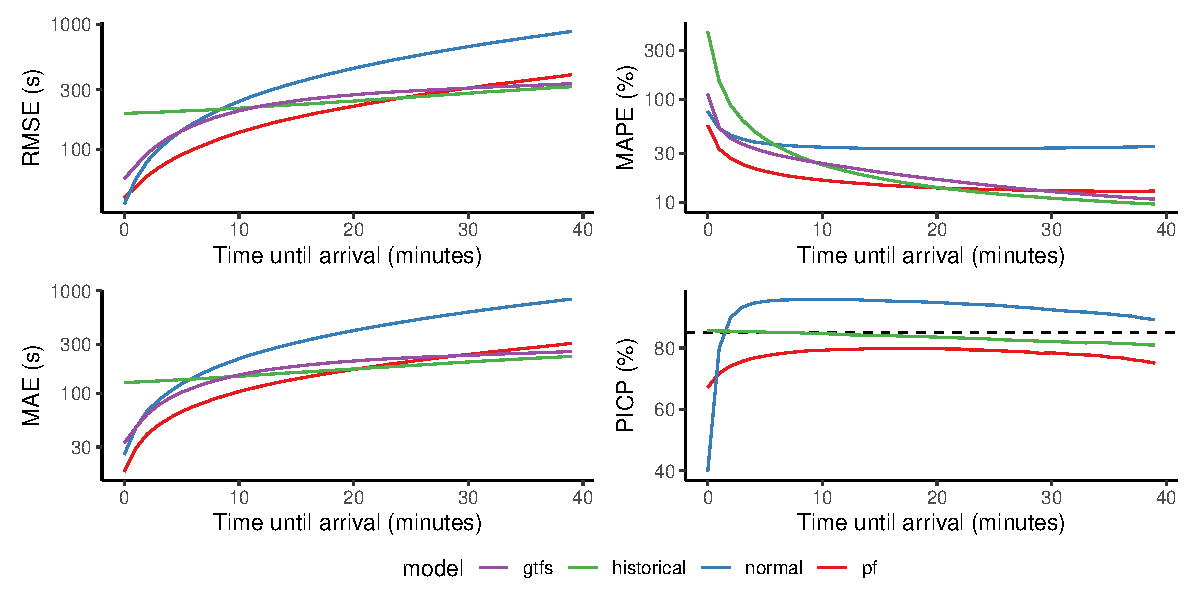
\includegraphics[width=\textwidth]{figure/model_results_rmse_time-1} \caption[Model comparative statistics as a function of time until arrival]{Model comparative statistics as a function of time until arrival.}\label{fig:model_results_rmse_time}
\end{figure}


\end{knitrout}



\subsubsection{Stop sequence}

Similarly to time until arrival, we grouped results by stop sequence---one being the first stop along the route---and computed \gls{rmse}, \gls{ppi} coverage and \gls{ppi} width, displayed in \cref{fig:model_results_rmse_stopn}. The \gls{rmse} increases for all models up until stop 40, after which point only few routes have that many stops, so there is increased variability between consecutive stops. All models show approximately the same error, besides $\FM_2$ as before. Method $\FM_1$ has the smallest error for the first 30 stops, after which point $\FM_4$ performs slightly better, but again the stop-to-stop variability here is larger.



\begin{knitrout}\small
\definecolor{shadecolor}{rgb}{0.969, 0.969, 0.969}\color{fgcolor}\begin{figure}
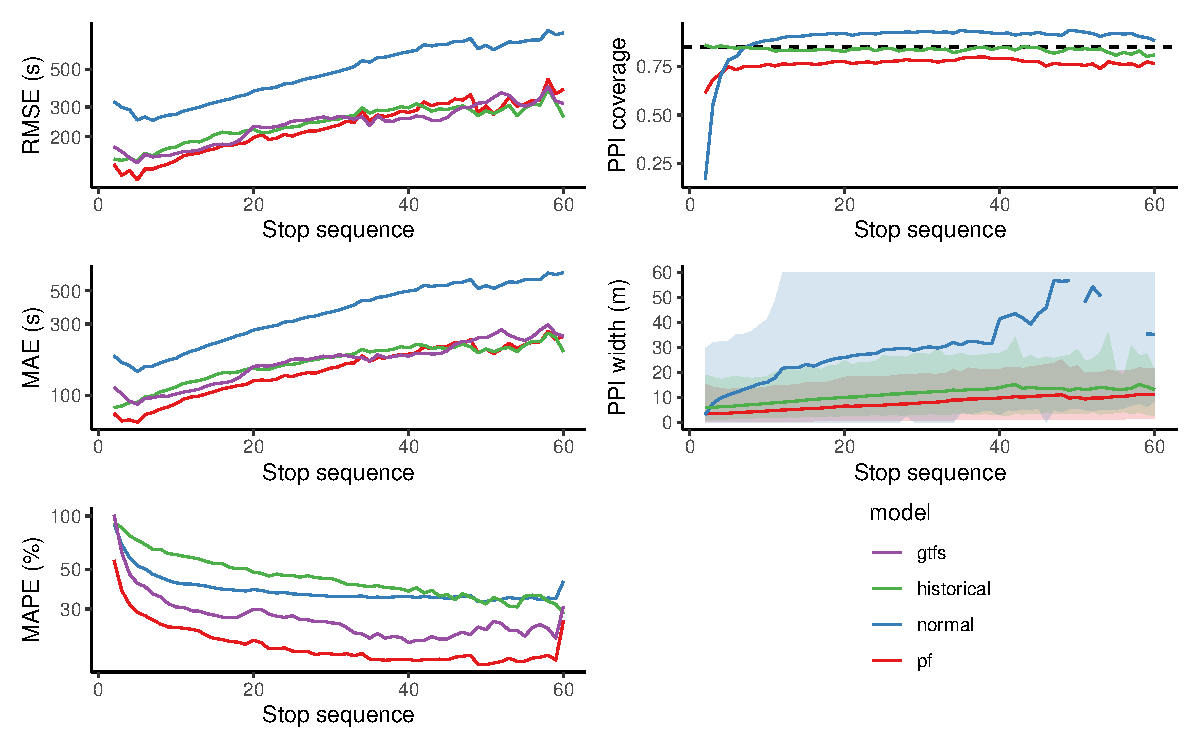
\includegraphics[width=\textwidth]{figure/model_results_rmse_stopn-1} \caption[Model comparative statistics as a function of stop sequence]{Model comparative statistics as a function of stop sequence.}\label{fig:model_results_rmse_stopn}
\end{figure}


\end{knitrout}

The \gls{ppi} coverage and width show much the same trend as before. This is not unexpected, since there is a relationship between time until arrival and stop sequence: low sequence stops do not ever have a long time until arrival. Method $\FM_1$ has a shorter interval width, but again this comes with lower coverage. The quantiles of observed \gls{ppi} width in \cref{fig:model_results_rmse_stopn3} again show little significant different between $\FM_1$ and $\FM_3$, while $\FM_2$ is again overestimating uncertainty.



\subsubsection{Time of day}

We grouped observations into 15~minute intervals over the day and calculated the summary statistics for each forecasting method. The results, displayed in \cref{fig:model_results_rmse_timeofday}, differ quite significantly from those seen previously, as we see a strong peak-hour effect\footnote{In the morning there is a single peak at around 8~am, whereas in the evening there are two peaks: one for schools at about 3~pm, and another for workers at around 5~pm.}.

In \cref{fig:model_results_rmse_timeofday1}, the prediction error is smallest for the particle filter method at all times \emph{except} during the morning and evening peaks, with the afternoon school peak showing a more considerable increase than the worker peak. Method $\FM_4$ also shows a slight increase at peak times, but it is far less significant. Similarly, $\FM_3$ shows increases at peak times, as well as another in the afternoon.


The coverage of the \glspl{ppi} for both $\FM_1$ and $\FM_3$ are, during the day time off-peak period (9h30--14h30), both close to 85\% (\cref{fig:model_results_rmse_timeofday2}), and we see that most of the particle filter's poor coverage comes from outside of this period. It is worth noting here that, though discussed in \cref{sec:nw_hist_model}, the historical data-based forecasting model has not yet been implemented, so there may yet be improvements in the particle filter's performance if it was able to forecast peak speed effects.





\begin{knitrout}\small
\definecolor{shadecolor}{rgb}{0.969, 0.969, 0.969}\color{fgcolor}\begin{figure}
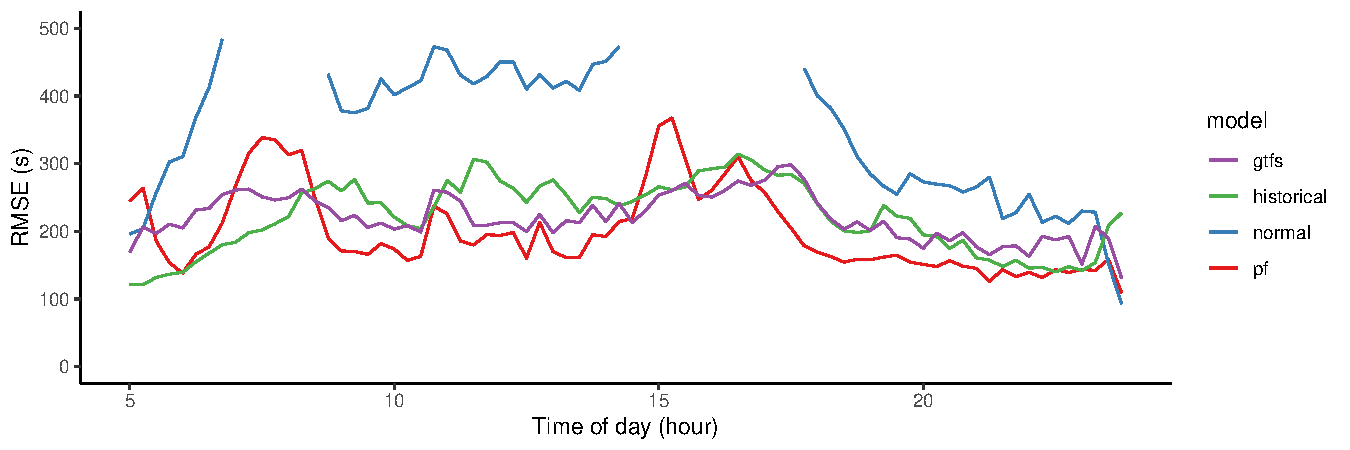
\includegraphics[width=\textwidth]{figure/model_results_rmse_timeofday-1} \caption[Model comparative statistics as a function of time of day]{Model comparative statistics as a function of time of day.}\label{fig:model_results_rmse_timeofday}
\end{figure}


\end{knitrout}

As for the interval widths, these are reasonably constant over the day, with a small increase at peak times for $\FM_1$ and $\FM_3$. There is no noticable difference in the widths for $\FM_1$ and $\FM_3$; however, again $\FM_2$ overestimates the uncertainty, leading to prediction interval widths of up to 40~minutes \emph{on average}.



\subsection{Comparing arrival probabilities and wait times}
\label{sec:prediction_model_comp_probs}

\Gls{rmse} is a simple measure of predictive performance but takes no account of the application and the cost of an inaccurate prediction. In our case, there are two costs we need to consider:
\begin{enumerate}
\item wait time at the bus stop, and
\item missing the bus altogether.
\end{enumerate}
Clearly, the latter---in most cases---incurs a much greater cost, but depends entirely on time until the \emph{next} bus arrival: for high-frequency routes, this is not a problem; for low-frequency ones, however, it is\footnote{Some routes only run hourly!}. In this section, we do not differentiate between high and low-frequency routes.


The three statistics we compare across the methods are:
\begin{itemize}
\item $\mathbb{P}_m = \Pr{\Varr_m \geq \hat\Tarr_m}$, the probability that the vehicle arrives after the point estimate, $\hat\Tarr_m$;
\item $\mathbb{P}_\ell = \Pr{\Varr_m \geq \hat\alpha_{m,\text{lower}}}$, the probability that the vehicles arrives after the lower bound of the \gls{ppi}; and
\item $\mathbb{E}_\ell = \E{\Varr_m - \hat\alpha_{m,\text{lower}} | \Varr_m \geq \hat\alpha_{m,\text{lower}}}$, the expected waiting time for a passenger arriving at the lower predictive bound, given that the bus arrives after it.
\end{itemize}


For the overall results, shown in \cref{tab:model_results_pr_miss}, we see that, if a passenger at any time looks at the \gls{eta} of their bus \emph{once} and arrives at the stop by the indicated time, then by $\FM_1$ their probability of catching the bus is almost double that of using the currently deployed method, $\FM_4$. Using historical data averages, then (not surprisingly) $\mathbb{P}_m$ is about 50\%; $\FM_2$ is over 95\% which indicates that it underestimates arrival times.


As for the lower quantile ($\mathbb{P}_\ell$), the probabilities are approximately the same. Since these are 5\% quantiles, we would expect the bus to arrive after it about 95\% of the time. As for the expected wait time, given arrival by the lower quantile and that the bus arrives after it, the particle filter has the shortest, while (as with the previous results) $\FM_2$ is over four times as long.


Perhaps the more relevant comparison, however, is between $\FM_1$ and $\FM_4$; however, since there is no \gls{ppi} available (the schedule-delay is just a single point estimate), we need another way to compare them. \Cref{fig:model_results_pr_gtfs1} shows, as dashed lines, the values of $\mathbb{P}_\ell$ from \cref{tab:model_results_pr_miss}, overlaid with a curve of the probability of catching the bus (y-axis) given a passenger arrives $x$ minutes before the displayed arrival time. We see that one would need to arrive a little over 6~minutes before the stated \gls{eta} for the same probability of catching the bus as the particle filter. In \cref{fig:model_results_pr_gtfs2}, we show the expected wait time, $\mathbb{E}_\ell$, given the passenger arrives before the lower limit for the three other methods (dashed lines) and the curve for arriving $x$ minutes before the stated time using $\FM_4$. Given arrival 6~minutes before the stated arrival time, the expected waiting time is about 6~minutes, a couple of minutes longer than the particle filter. The inverse would be, for an equivalent expected waiting time for both $\FM_1$ and $\FM_4$, one would need to arrive four minutes before the $\FM_4$-forecasted arrival time (\cref{fig:model_results_pr_gtfs2}), which corresponds to an 80\% chance of arriving before the bus does (\cref{fig:model_results_pr_gtfs1}).


For the remainder of this section, we use 6~minutes before the specified \gls{eta} to obtain a lower bound for $\FM_4$, and compare the probabilities as a function of time until arrival, stop sequence, and time of day.



\begin{knitrout}\small
\definecolor{shadecolor}{rgb}{0.969, 0.969, 0.969}\color{fgcolor}\begin{table}

\caption{\label{tab:model_results_pr_miss}The probability of catching a bus given a passenger arrives by the mean/median ($\mathbb{P}_m$) and lower quantile ($\mathbb{P}_\ell$), along with the expected waiting time, in minutes, given arrival by the lower quantile, for each of the for forecast methods.}
\centering
\fontsize{8}{10}\selectfont
\begin{tabular}[t]{lrrrl}
\toprule
  & $\mathbb{P}_m$ & $\mathbb{P}_\ell$ & $\mathbb{E}_\ell$ (m) & (95\% CI)\\
\midrule
$\mathcal{F}_1$: Particle filter & 0.64 & 0.93 & 4.45 & (0.2, 16.6)\\
$\mathcal{F}_2$: Normal approximation & 0.96 & 0.98 & 20.90 & (1.2, 63.7)\\
$\mathcal{F}_3$: Historical delays & 0.54 & 0.98 & 7.13 & (0.7, 20.8)\\
$\mathcal{F}_4$: Schedule-delay & 0.38 &  &  & \\
\bottomrule
\end{tabular}
\end{table}


\end{knitrout}

\begin{knitrout}\small
\definecolor{shadecolor}{rgb}{0.969, 0.969, 0.969}\color{fgcolor}\begin{figure}

{\centering 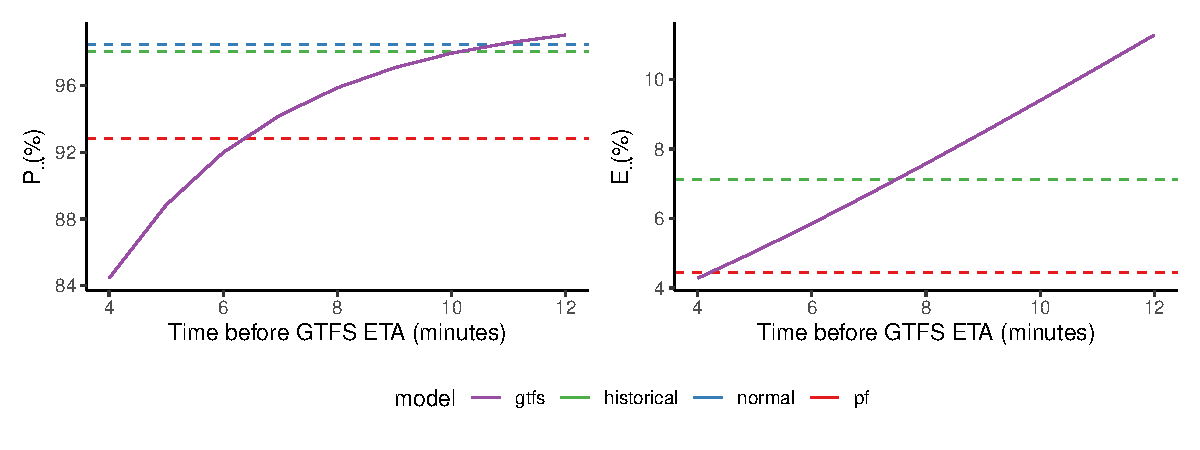
\includegraphics[width=\textwidth]{figure/model_results_pr_gtfs-1} 

}

\caption[GTFS equivalent]{GTFS equivalent}\label{fig:model_results_pr_gtfs}
\end{figure}


\end{knitrout}


\subsubsection{Time until arrival}

\Cref{fig:model_results_pr_time} shows $\mathbb{P}_m$, $\mathbb{P}_\ell$, and $\mathbb{E}_\ell$ computed in one-minute intervals for each of the four models. We see that the probability that the vehicle arrives after the estimate is reasonably constant, with a slight decrease as the bus nears the stop; however, the four methods are distinct from each other, yielding the same conclusion as before \textcolor{red}{(be more specific)}.

As for $\mathbb{P}_\ell$, displayed in \cref{fig:model_results_pr_time2}, we see a different trend: $\FM_1$ and $\FM_3$ increase the further out the vehicle is, while in $\FM_4$ the probability decreases. Clearly, this is because we have chosen a fixed lower bound. When the vehicle is less than 15 minutes out, arriving 6~minute before the schedule-delay estimate results in a higher probability of catching the bus than the particle filter because the width is greater.


Finally, we look at the expected waiting time, given a passenger arrives at the lower bound \emph{and} the bus arrives sometime after, which is displayed in \cref{fig:model_results_pr_time}. The particle filter has a consistently shorter waiting time, though by about 30~minutes out the three methods excluding the normal approximation are approximately the same. We can see that the expected waiting time for $\FM_4$ is more or less independent of time until arrival.



\begin{knitrout}\small
\definecolor{shadecolor}{rgb}{0.969, 0.969, 0.969}\color{fgcolor}\begin{figure}
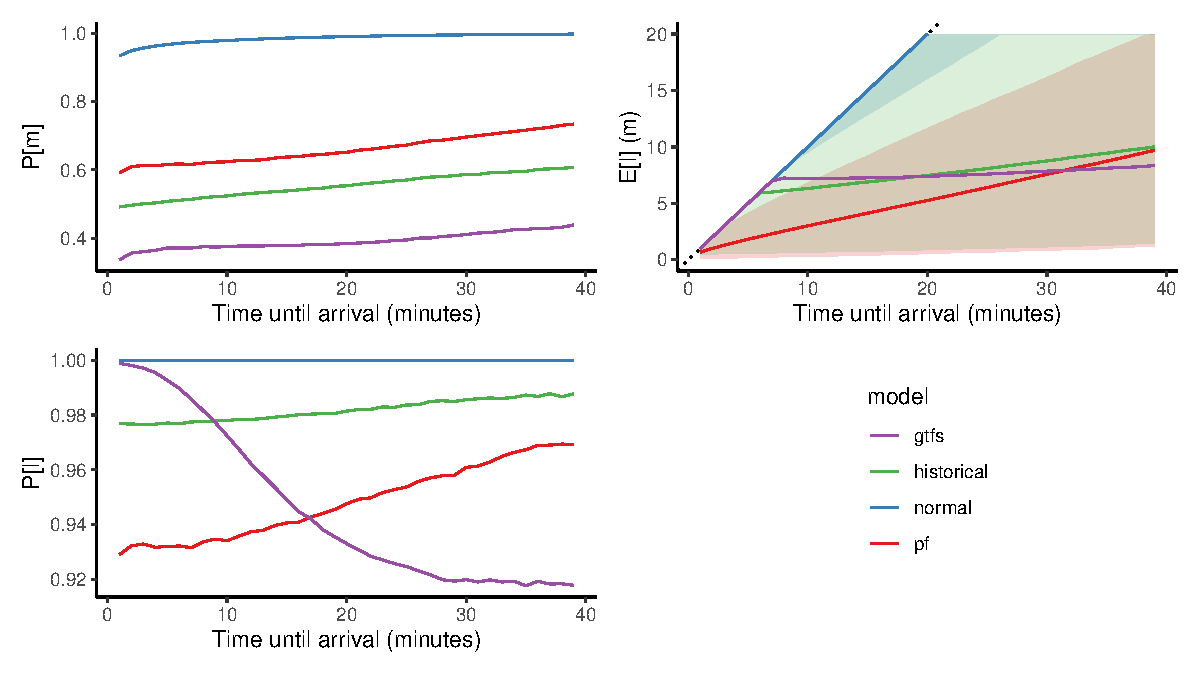
\includegraphics[width=\textwidth]{figure/model_results_pr_time-1} \caption[Summary values by time until arrival]{Summary values by time until arrival.}\label{fig:model_results_pr_time}
\end{figure}


\end{knitrout}


\subsubsection{Stop sequence}

Next, we computed the same values by stop sequence, as is shown in \cref{fig:model_results_pr_stop}. For most stops, the particle filter has a higher probability of the bus arriving after the point estimate ($\mathbb{P}_m$), though for early stops this is not the case. However, this is simply because the particle filter \emph{does not make a prediction} until the vehicle has been observed\footnote{Yet! Future work will work to use historical data in this situation}, whereas the \gls{gtfs} approach assumes the delay is zero until the vehicle is observed. This assumption can be reasonably accurate, particularly for the first few stops when there has not been enough time for the bus to get behind or ahead of schedule.

The trend for $\mathbb{P}_\ell$ is similar to what we saw with time until arrival. This time, however, the particle filter has much lower probabilities for the first few stops, again due to the reasons stated above. Even so, $\FM_4$ is consistently higher than $\FM_1$ until stop 40. The expected waiting time again shows better performance with the particle filter method until about stop 40, after which point the methods are more or less the same, given not many routes have over 40~stops. There is a trade-off here between waiting time and catch probability.


\begin{knitrout}\small
\definecolor{shadecolor}{rgb}{0.969, 0.969, 0.969}\color{fgcolor}\begin{figure}
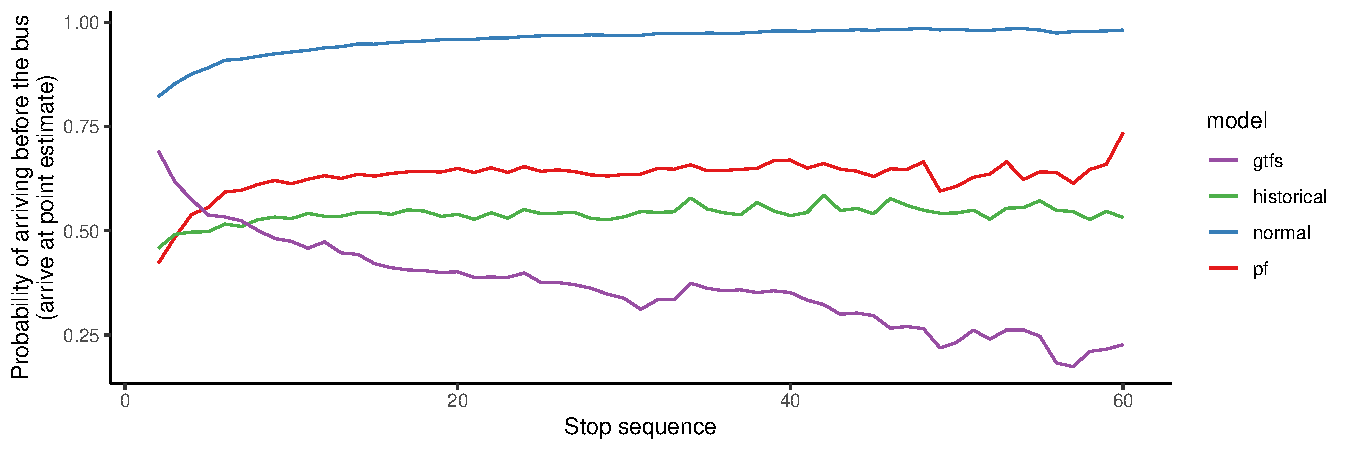
\includegraphics[width=\textwidth]{figure/model_results_pr_stop-1} \caption[Summary values by stop sequence]{Summary values by stop sequence.}\label{fig:model_results_pr_stop}
\end{figure}


\end{knitrout}


\subsubsection{Time of day}

Calculating the probabilities and expected waiting time in 15~minute intervals for each of the models is shown in \cref{fig:model_results_pr_timeofday}, in which the peak hour effects are visible, associated with an increased probability of arriving before the bus does in the particle filter method for both the median and lower bound. The schedule-delay method is negatively affected by peak hour in the lower bound estimate. The historical data estimate shows little effect due to peak hour but performs better in the day time (versus early morning and late evening).


For the expected waiting time, the particle filter is overall the lowest, even during peak where it shows a significant increase, seen in \cref{fig:model_results_pr_timeofday3}. The historical and schedule-delay methods both have similar expected waiting times of about 6--7 minutes.


\begin{knitrout}\small
\definecolor{shadecolor}{rgb}{0.969, 0.969, 0.969}\color{fgcolor}\begin{figure}
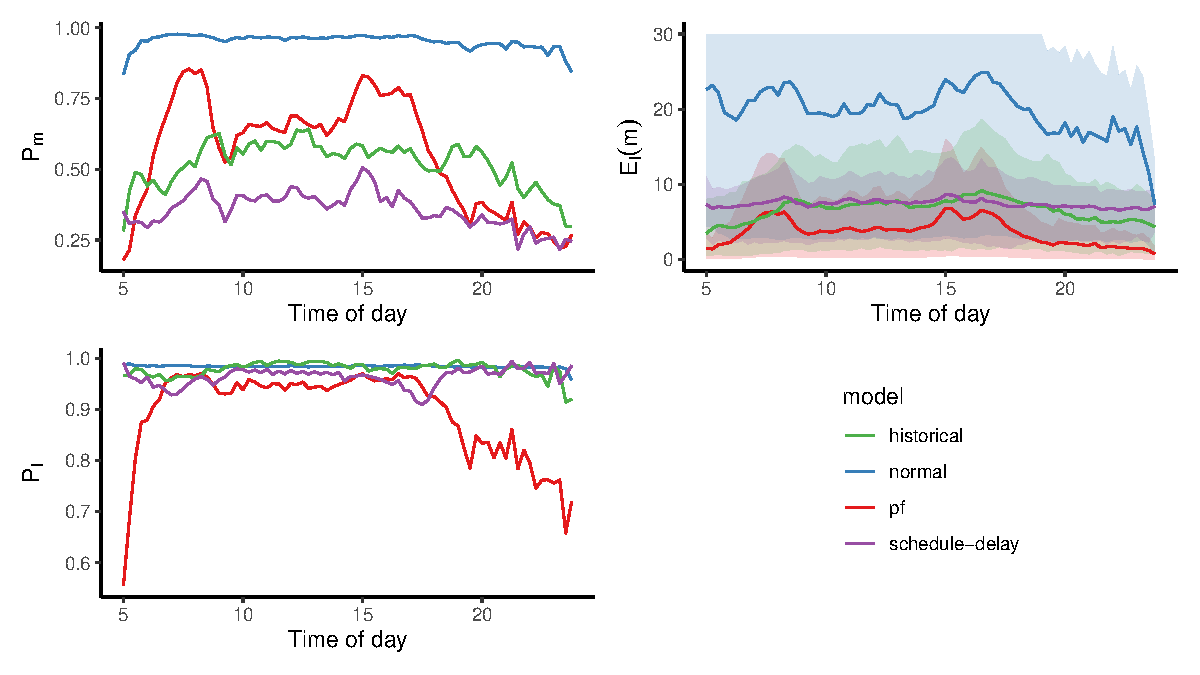
\includegraphics[width=\textwidth]{figure/model_results_pr_timeofday-1} \caption[Summary values by time of day]{Summary values by time of day.}\label{fig:model_results_pr_timeofday}
\end{figure}


\end{knitrout}



\subsection{Result summary}
\label{sec:prediction_model_comp_summary}

We have now seen that the particle filter suggests some improvement is possible over the schedule-delay method used by \AT. It tends to underestimate the arrival time, but even so, the expected waiting time is, in most situations, less than that of all of the other methods. Conversely, the normal approximation performed very poorly in this case, likely since summing uncertainties, and assuming independence, quickly results in an overestimation of uncertainty, and thus wide prediction intervals (not to mention high prediction error).

As for the other methods which do not use real-time network information, the historical data-based method performed as well as or better than the schedule-delay method, with a few situations where it did not perform so well. The average and variance of arrival delays were based on two weeks' worth of data, which is---at most---10 observations per trip. Processing more weeks of data could bring slight improvements, but without taking into account real-time data, it is unlikely to yield significant improvements. Post-processing is an intensive procedure, so future development could include real-time computation of the mean and variance of arrival time for each stop along each trip.
